% 茅台年报 RAG 问答系统 · 项目技术报告
% 编译: tectonic -o report/_build report/report.tex
\documentclass[UTF8,11pt]{ctexart}
\usepackage[margin=2.4cm]{geometry}
\usepackage{graphicx}
\usepackage{booktabs}
\usepackage{amsmath}
\usepackage{float}
\usepackage{hyperref}
\usepackage{xcolor}
\hypersetup{colorlinks=true, linkcolor=blue!60!black, urlcolor=blue!60!black}

\title{\textbf{给年报装上"提问"功能：\\茅台年报 RAG 问答系统的搭建与评测}}
\author{项目技术报告}
\date{2026年10月}

\begin{document}
\maketitle

\begin{abstract}
年报名厚、术语多，想确认一个数字往往要翻几十页。本项目把贵州茅台
2022--2025 年四份年度报告（共 556 页）做成一个"能提问的资料库"：用自然
语言提问，系统先去年报里\textbf{检索}最相关的段落，再让大模型\textbf{只根据这些
段落}生成答案，并且\textbf{每条答案都标注出处页码}。我们建立了 50 题的黄金
评测集，把系统效果变成可以复现的数字，并通过切块策略、检索方式、精排模
型、生成模型四组对照实验说明每一项改进带来了多少提升。
\end{abstract}

\tableofcontents

\section{我们要解决什么问题}

\textbf{一句话：}把``翻半小时 PDF 找一个数''变成``问一句，十秒拿到带原文出处的答案''。

这个系统的目标用户是个人投资者和研究者。他们的真实场景是：持股人想核对
``今年分红方案和去年比怎么样''；研究员想快速确认``直销渠道占比的变化''。
这些问题本身不难，难的是\emph{找}——答案散落在几百页的表格和附注里。

需要说明的是，本系统\textbf{不提供投资建议}，也\textbf{不替用户做判断}，它只做两件
事：找得准（检索）、说得实（答案严格来自原文并附出处）。查不到就明说查
不到，绝不编造。

这套方法的真正价值在于\textbf{可迁移}：把年报换成员工手册、法规汇编、产品说
明书，就是一套企业知识库问答的原型。年报只是我们选定的``练兵场''——它公开
合法、答案可以在海量新闻中交叉验证、而且表格密集足够难。

\section{RAG 是什么：先查资料，再回答}

大模型（如 Qwen、DeepSeek）很聪明，但有两类天然的毛病：训练数据里没有
你的私有资料；而且被问到不知道的事时，倾向于\textbf{编一个像样的答案}
（即``幻觉''）。

RAG（Retrieval-Augmented Generation，检索增强生成）的思路非常朴素：
\textbf{回答之前，先把相关资料查出来，塞给模型，让它照着资料说话。}
整个流程分五步（图~\ref{fig:pipeline}）：

\begin{enumerate}
  \item \textbf{切块}：把 556 页年报切成约 500 字的小段（共 1761 块），
        每块记住自己来自哪一年第几页；
  \item \textbf{向量化}：用一个中文嵌入模型（BGE）把每块文字变成 512 个
        数字的向量——意思相近的文字，向量距离也近；
  \item \textbf{建索引}：所有向量存成一张表，支撑``找最近''的运算；
  \item \textbf{检索}：用户提问时，把问题也变成向量，找出最相似的 5 块；
  \item \textbf{生成}：把问题与这 5 块原文一起交给大模型，要求答案必须
        标注出处、查不到就承认。
\end{enumerate}

一个直观的类比：向量检索像\textbf{搜索引擎}（找字面上最相似的段落），
而系统维护的``哪块文字来自哪一页''的记录，让每条答案都能像论文一样
给出``参考文献''。

\begin{figure}[H]
  \centering
  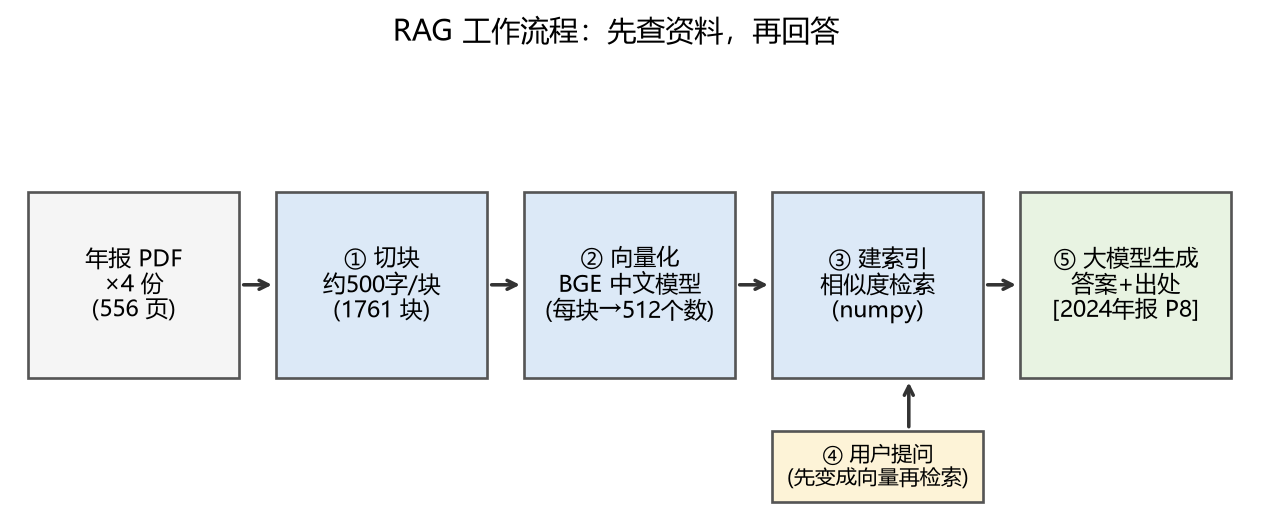
\includegraphics[width=0.95\textwidth]{figures/fig_pipeline.png}
  \caption{RAG 五步流程：先查资料，再回答。用户问题（④）进入检索，
  系统把最相关的段落连同问题一起交给大模型生成答案（⑤）。}
  \label{fig:pipeline}
\end{figure}

\section{数据长什么样，难在哪}

语料为巨潮资讯网公开披露的贵州茅台 2022--2025 年年度报告（中文完整版），
四份共 556 页、约 63 万字符。PDF 自带文本层，无需 OCR，逐页提取即可，
且 PDF 页码与印刷页码一致——这让``P8''这样的出处标注可以直接验证。

年报文本有三个典型的难点，也是评测中真实出现的``病例''：

\begin{itemize}
  \item \textbf{表格被切碎}：提取后的表格单元格按行折断，
        例如``分渠道营收''表的表头被拆成``本期期 / 末数占 / 总资产 / 的比例''
        四行，语义支离破碎；
  \item \textbf{同一内容多处出现}：``营业总收入''同时出现在经营讨论
        （P8）、财务报表（P9）、附注（P56），版本与口径并不相同；
  \item \textbf{年份混淆}：四年报告结构高度相似，``2023 年销售费用''的
        提问很容易召回 2024 年的同名段落——字面相似度极高，
        语义上却是另一年的事实。
\end{itemize}

这些病例决定了后面实验的设计：切块策略针对表格切碎，混合检索针对字面
匹配，而年份识别针对年代混淆。

\section{系统怎么搭}

\textbf{总体选型原则：}每个环节用最简单可靠的方案，把复杂度留给评测与
实验。全部运行在本地（除对比实验调用云端 API 外），单机 RTX 5070 +
32GB 内存即可。

\begin{table}[H]
\centering
\begin{tabular}{llp{7.2cm}}
\toprule
环节 & 选型 & 理由 \\
\midrule
切块 & 按页 500 字窗口、重叠 100 字 & 不跨页切块，保证出处精确到页 \\
向量化 & BGE-small-zh-v1.5（本地） & 中文效果好的开源小模型，CPU 即可 \\
索引/检索 & numpy 暴力余弦 & 仅 1761 块，单次检索 $<$1ms；语料达百万级
再引入专业向量库。曾尝试 Chroma，其在 Windows 上存在持久化缺陷
（写入后无法重开），故弃用 \\
生成模型 & Qwen3-4B（Ollama，本地） & 12GB 显存可流畅运行；另有云端
模型参与对比实验 \\
界面 & Streamlit & 对话问答 + 出处展开 + 双年报对比 \\
评测 & 自研确定性指标 & 黄金集每题带标准出处页，检索是否命中可直接
程序判定，不依赖模型打分 \\
\bottomrule
\end{tabular}
\caption{系统各环节选型}
\end{table}

\textbf{工程上的两个决定值得说明。}其一，\emph{不跨页切块}：牺牲了少量
语义完整性，换来每块出处严格精确到页——对``答案必须可溯源''这一目标，
这是更划算的交换。其二，\emph{自研评测指标而非直接套用 ragas 等框架}：
检索层指标（是否命中出处页）是确定性的，程序判定比让另一个大模型打分
更可复现、零成本；答案层的忠实度打分如需主观判定，才引入模型评分。

\section{实验与结果}

\subsection{评测集}

50 题，人工核对答案与出处页：30 道单页事实题、10 道跨页/跨表题、
5 道跨年份对比题、5 道\textbf{年报里根本没有答案}的题（考察系统是否
会``不懂装懂''）。

\subsection{基线：一半以上的问题查不准}

检索层基线成绩（k=5，即每次给模型 5 段参考资料）：

\begin{table}[H]
\centering
\begin{tabular}{lcccc}
\toprule
题型 & 题数 & 出处页命中率 & MRR & 命中精确率 \\
\midrule
事实题 & 30 & 36.7\% & 0.179 & 7.3\% \\
跨页题 & 10 & 30.0\% & 0.250 & 6.0\% \\
跨年题 & 5  & 20.0\% & 0.200 & 4.0\% \\
无答案题 & 5 & 0.0\% & 0.000 & 0.0\% \\
\midrule
\textbf{总览} & 50 & \textbf{30.0\%} & \textbf{0.177} & \textbf{6.0\%} \\
\bottomrule
\end{tabular}
\caption{基线检索成绩（数据来自 results/baseline\_retrieval.json，脚本可复现）}
\label{tab:baseline}
\end{table}

\begin{figure}[H]
  \centering
  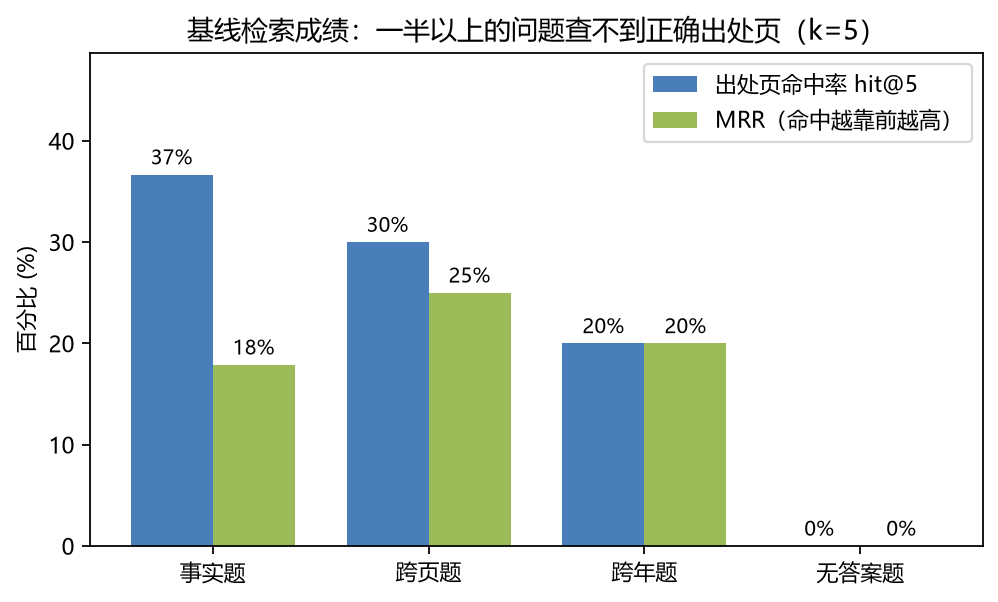
\includegraphics[width=0.85\textwidth]{figures/fig_baseline.png}
  \caption{基线检索成绩：只有三成的问题检索到了正确出处页}
  \label{fig:baseline}
\end{figure}

30\% 的命中率意味着：大多数情况下，模型拿到的参考资料里\textbf{根本没有
正确答案所在的那一页}。逐题分析未命中样本，病灶有三类，按出现频率排序：

\begin{enumerate}
  \item \textbf{年份混淆}（最严重）：``2023 年营业总收入''召回了 2024 年
        P8 的同类段落——两段文字几乎一样，只是年份不同。嵌入向量对
        ``数字年份''的敏感度远低于对``业务词汇''的敏感度；
  \item \textbf{同主题错页}：``2022 年末员工人数''召回了 2022 年 P42
        （员工专业结构），而数字在 P30（员工情况表）——同章节内
        相邻页的区分度不足；
  \item \textbf{同主题错章节}：``分红方案''召回了后文的``利润分配''章节
        （P32--33），而标准答案在卷首``重要提示''（P2）——年报里
        同一信息出现多处，检索只能``押中''其中一处。
\end{enumerate}

这三类病灶直接决定了下面的实验设计。

\subsection{实验一：切块策略（E1）}

% TODO: E1 结果表格（固定500字 vs 结构化切块 vs 父子块），跑完后填入
（待实验完成后填入）

\subsection{实验二：检索方式（E2）}

% TODO: E2 结果（纯向量 vs 向量+BM25混合+年份识别过滤）
（待实验完成后填入）

\subsection{实验三：精排（E3）}

% TODO: E3 结果（bge-reranker 前后对比 + 延迟代价）
（待实验完成后填入）

\subsection{实验四：生成模型能力（E4）}

% TODO: E4 结果（本地 Qwen3-4B vs DeepSeek API，同一检索配置）
（待实验完成后填入）

\subsection{典型病例分析}

% TODO: 2-3 个 badcase 的完整问答展示（改进前 vs 改进后）
（待实验完成后填入）

\section{边界与结论}

\textbf{系统的边界，和它做到的事一样重要：}

\begin{itemize}
  \item 它\textbf{不会算术}：``毛利率下降了几个百分点''这类需要两数相除的
        问题，纯检索容易失败——答案里需要出现的两个数可能分别检索成功，
        但计算步骤可能出错。评测集刻意不考计算，报告以``两个数各自
        是否找到''为准；
  \item 它\textbf{只懂年报截止日之前}的世界：问``最新股价''必然无法回答；
  \item 无答案题的表现是\textbf{信任的底线}：系统对年报里没有的信息必须
        明确说``无法回答''，这一指标在答案层评测中单独统计。
\end{itemize}

% TODO: 结论段（四组实验的总结论、最有价值的发现、下一步方向），实验完成后填入

\appendix
\section{复现指南}

\begin{enumerate}
  \item 环境要求：Windows / Python 3.12，NVIDIA 显卡可选（仅加速本地
        大模型推理，检索与嵌入 CPU 即可）；
  \item 数据：\texttt{python scripts/download\_data.py}（巨潮资讯网公开文件）；
  \item 建索引：\texttt{python scripts/extract\_text.py \&\& python scripts/build\_index.py}；
  \item 问答：\texttt{python -m src.ask "你的问题"} 或
        \texttt{python -m streamlit run src/app.py}；
  \item 评测：\texttt{python scripts/evaluate\_retrieval.py} 与
        \texttt{python scripts/evaluate\_answers.py}；
  \item 报告编译：\texttt{tectonic -o report/\_build report/report.tex}。
\end{enumerate}

\end{document}
